\section{Parallel Strategy and Performance}

\subsection{Parallel Strategy}

% GB to work on this
%  - expand to include better description
%  - include load balancing options

When \enzo\ is run on a distrubuted platform, some of the data is
replicated to all processors, while some remains on a single processor.
A description of the entire hierarchy (the position and size of each grid, as well
some other meta data) is stored on each processor.  This enables each
grid to know what grids are near it in the hierarchy, regardless of
where the data is.  The actual Baryon data (density, velocity, energy,
and any chemistry data) and particle data are stored on only one
processor.  Storing the entire hierarchy on all processor does create
some overhead, but in practice this is not an issue until one reaches
the extremely large scale.
  The code handles load balancing 
on a level-by-level basis such that the workload on each level is 
distributed as uniformly as possible across all processors.  Spatial locality of 
grids is not forced during message passing, for maximum flexibility (though not
necessarily maximum efficiency).  
The MPI message passing library\footnote{http://www-unix.mcs.anl.gov/mpi/}
 is used to transfer data between processors.
 
 


%old text
%Every processor 
%keeps a description of the entire grid hierarchy at all times, so that 
%each processor knows where all grids are.  However, baryon and particle 
%data for a given grid only exists on a single processor.  See 
%Figure~\ref{fig.2.amrhierarchy} for a schematic example of this.  



\begin{figure}
\begin{center}
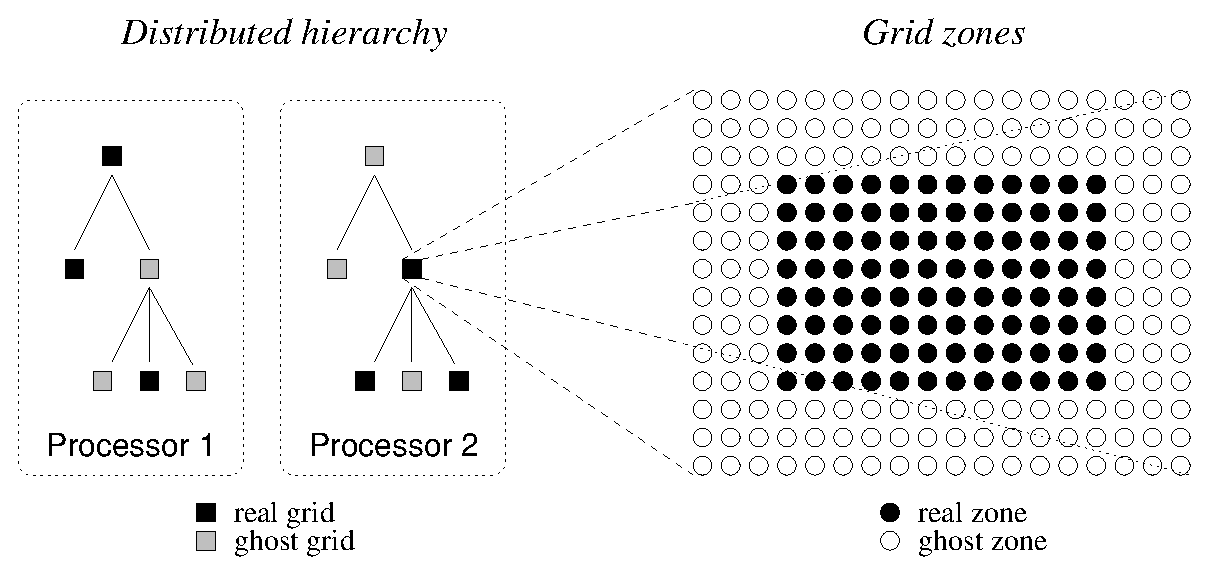
\includegraphics[width=0.4\textwidth]{figures/amr_hierarchy.eps}
\end{center}
\caption{\emph{Left:}  Example of a simple, distributed AMR hierarchy showing real and ghost grids.
\emph{Right:}  Example 2D \enzo\ grid showing real and ghost zones, as 
needed for the PPM hydro stencil. }
\label{fig:amr_hierarchy}
\end{figure}



% ----------------------------------

\subsection{Performance}
\label{sec.performance}

\subsubsection{Performance model \red{(Greg)}}

% Maybe include Greg's text on general scaling arguments

\subsubsection{Performance Measurement \& Instrumentation \red{(Sam)}}

Because of the wide variety of simulations, methods, and uses of \bb{enzo}, it
is difficult to define exactly which routines are most costly during a given
simulation.  As such, we have designed a lightweight registering system that
has been implemented for the most commonly used routines (such as the
hydrodynamic and gravity solvers) as well as refinement level timers that
measure the (exclusive) time spent on each level.  Beyond this minimal set of
routines, we have designed a simple way for the user to modify the source
by adding TIMER_START(``Your Routine Name'') and TIMER_END(``Your Routine
Name'').  These timers are automatically registered in a
std::map\footnote{http://www.cplusplus.com/reference/map/map/}.  These timers
are created and managed individually on each processor in an asynchronous
fashion.  

At each complete EvolveHierarchy (or less often if specified), each timer is
then communicated to the root processor where it calculates the mean, standard
deviation, minimum, and maximum for each of the timers across all processors. 
For level timers, there are also attributes such as the number of cell updates,
the current number of grids, and the average cells/s/MPI process.  This
information is then output to a ``performance.out'' logfile.  This provides a 
simplified interface to the user that can be used to diagnose performance 
issues as well as estimate a given problem type's scalability.  In addition to 
the logfile, we have developed a plotting interface for quickly producing 
figures that process the data from the logfile.  These capabilities are 
described in the online documentation, along with a further discussion of the 
performance measurement implementation.

\subsubsection{Unigrid scaling \red{(Brian)}}

% Brian to work on this, scaling data from Harkness

\subsubsection{AMR scaling \red{(Greg)}}

% Greg to work on this, scaling data from his runs, or maybe from John Wise
